\pagestyle{fancy}
\fancyhf{}
\fancyfoot[L]{\textbf{ECEN 4638--T.D. Murphey}}
\fancyfoot[R]{\textbf{Lab \#2}}
\fancyfoot[C]{\vspace{.2in}\thepage}
%\pagestyle{myheadings}
%\markright{ECEN 4638--T.D. Murphey \flushright Lab $\#1$}


\chapter{Lab \#2:  Digital Simulation of Torsional Disk Systems in
  LabVIEW}
\date{}
\maketitle
\thispagestyle{fancy}
%\thispagestyle{empty}

\begin{center}  \textbf{Objective}
\end{center}

The purpose of this lab is to increase your familiarity with LabVIEW, increase
your mechanical modeling prowess, and give you simulation models that you can
use to verify your designs before testing them on hardware.  

The model you write today will allow you to to simulate what the Torsional Disk
System (TDS) will do in response to a given input.  However, this response is
dependent on the value of certain parameters for the system, such as the
rotational inertia of the disks, the torsional spring constants, and the
dissipation due to bearings and gears.  These parameter values will have to
estimated using a process called \emph{system identification}.  (You will do
this heuristically in this lab and will do it more formally in Lab \#3.)
Although system identification can involve no modeling whatsoever, it is almost
always easier to do it when one is only trying to estimate a finite number of
parameters.  Hence, it is generally better to think of modeling and system
identification as being inter-dependent.  Once you have a model that is
reasonably accurate, you will finally be in a position to do some actual control
design (which will start in Lab \#4).

It is worth noting that this is roughly the cycle that you would go through if
you were doing an actual industrial project.  This cycle is generally 1) Model,
2) Verify Model Experimentally, 3) Design Using Model, and finally 4) Test
Control Design Experimentally.  In general, no one would allow you to try
something out experimentally until you could show that the simulations indicate
it should work (or at least this is typically true).

\begin{center} \textbf{Lab Overview}
\end{center}

First, you need to find a model for the torsional disk system.  As you know, it
has three disks with different inertias and dissipation, and a torsional rod
that can be twisted to some degree, but has a linear torsional spring constant
associated with it that (along with dissipation in the system) relaxes each disk
back into its original orientation.  It is driven by a DC motor that you can
think of as directly applying a torque to the system, where the torque is scaled
by some factor $X$.

Second, you will need to show that you can create a simulation for one disk, two
disks, or all three disks.  You can be as clever as you want in terms of how you
program this.  However, I would suggest using a MathScript node in the
simulation module, such as Fig.~\ref{fig-mathscriptinsimTF}.  

Lastly, you will investigate what goes right/wrong with various feedback control
approaches.  This is largely intended to give you an appreciation of why we
think of control \emph{design} as actually being quite important!

\section{Pre-Lab Tasks}

The pre-lab requirements are roughly as follows:
\begin{enumerate}
\item Read this entire document
\item Prepare a model for the Torsional Disk System.  This will be a
  $2^{\textrm{nd}}$-order differential equation of three variables.  Be prepared
  to discuss your modeling with your teammates.  (It is unlikely that you will
  all arrive with the same model.)
\item Based on simulations, guess the parameters for the Torsional Disk System.
%\item Learn how to use the Symbolic Transfer Function (as noted at the end of
%  this lab).  
\end{enumerate}


\section{Tasks}


The torsional disk system has three disks of inertia $(J_1,J_2,J_3)$ (due to the
disks themselves and the masses we afix to the disks), damping coefficients
$c_1,c_2,c_3$ (due to friction in the bearings and other components supporting
the disks), a torsional rod connecting all three with torsional spring constants
$k_1$ and $k_2$ in between the disks, and a torque scaling constant $k_m$ that
scales signals (voltage) from the FPGA to the output torque of the motor.  When
doing system identification, these are the parameters you will need to be able
to identify in the next lab.  However, in order to identify them, you need a
model describing how the system behavior changes as one modifies the parameters.




\subsection{Task \#1--Mechanical Model}

\noindent \textbf{Task:} Based on what you have learned in class, find 
a model for this system.  Let the configuration variables of the bottom disk,
middle disk, and top disk be $(\theta_1,\theta_2,\theta_3)$ respectively (with their positive
directions measured by the right hand rule with the z-axis going up), the
moments of inertia be $J_1,J_2,J_3$, the viscous dissipation coefficients be
$c_1,c_2,c_3$ (i.e., with $\tau=-c_i \dot{\theta}_i$), and the spring constants between
disk 1 and 2 be $k_1$ (i.e., $\tau=-k_1(\theta_1-\theta_2)$) and between disk 2 and 3 be
$k_2$ (i.e., $\tau=-k_2(\theta_2-\theta_3)$).  Be sure to be careful with your sign
conventions!  Lastly, let the input torque from the motor be $T$.

\noindent \textbf{Task:}  What are the input, state, and output choices we have for this system?

\noindent \textbf{Task:}  How might you check to see if your sign conventions
are correct?

\begin{wrapfigure}[15]{r}{2in}
%\begin{figure}[h!]
\begin{center}
\vspace{-.1in}
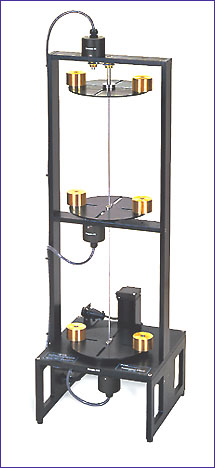
\includegraphics[height=4in]{Lab2/model205}
\end{center}
\vspace{-.15in}
\caption{The ECP Torsional Disk System.}
\label{fig-ecp}
%\end{figure}
\end{wrapfigure}


\noindent \textbf{Task:} What do you think are reasonable values of each of
these values?  You should be able to approximate this analytically for the
inertia (for a given set of masses attached to the disk).  The other parameters
you will have to guess, although you should defend your answer (partially by
noting whatever units you are using).  As you think about defending your choice
of parameters, you should think about what these choices would mean for the
actual physical system that we have in the lab.  For instance, you saw me twist
the two disks relative to each other, so you know that the spring constant
cannot be too high.  Thinking about physical units might also be helpful in
considering your guesses. What else do you know?  You will have a chance in a
moment to update your answer based on simulations.



\vspace{.2in}
\begin{tabular}{||l|l||}
\hline
Variable & \hspace{2in}Value \\
\hline
$J_1$ & \\
\hline
$J_2$ & \\
\hline
$J_3$ & \\
\hline
$c_1$ & \\
\hline
$c_2$ & \\
\hline
$c_3$ & \\
\hline
$k_1$ & \\
\hline
$k_2$ & \\
\hline
\end{tabular}
\vspace{.2in}

\noindent \textbf{Task:}  What are we \emph{not} modeling?  So far, we have only
included rigid body effects--what are other effects that might influence the
behavior of the system.  List three other effects you believe would most
influence the system that we have \emph{not} included in our mathematical
description of the system.

\noindent \textbf{Task:} Write the model both in state-space form and as a 
transfer function for all $\theta_i$ outputs.  you may wish (in fact, I highly
recommend) using a symbolic software package such as \emph{Mathematica} to
compute the transfer function from the state space model.

\subsection{Task \#2--Simulation}

\noindent \textbf{Task:} Implement your model both as a transfer function 
and as a state-space system in LabVIEW's Simulation Module.  You should
initially use the parameters that you have guessed, but you should be prepared
to change these parameters.  (If you do not have a transfer function at this
point, you should do the rest of the lab first using a state space model\textendash you can
create and use the transfer function outside of class if necessary.)

\noindent \textbf{Task:} Give the (open-loop!) model a step input.  Does the
model respond the way you expect it to?  You may, if you wish, come up and
experiment by hand with the torsional disk systems (while they are turned off).

\noindent \textbf{Task:} Start the simulation of your model at a
nontrivial initial condition (in the state-space model) to see if that tells you
anything else useful.  

\noindent \textbf{Task:} How can other measurements help you, such as:  
natural frequency of oscillation, rate at which the system response decays due
to dissipation, and sluggishness of response of the system to input torque?  Can
you think of anything else that would allow you to evaluate the correctness of
your model?

\noindent \textbf{Task:} For each case, turn in a plot that includes the
relevant \emph{output} of the system and the input, explaining what the result
implies for your choice of parameter.  

\begin{center}
\framebox{\parbox{4in}{Note that this part of the lab is very open-ended.  It is intended to be
open-ended.  Don't get frustrated!}}
\end{center}

\noindent \textbf{Task:} Now, based on your findings, choose different 
(or possibly the same, if you were very lucky) parameters of the system
\begin{center}
\begin{tabular}{||l|l||}
\hline
Variable & \hspace{2in}Value \\
\hline
$J_1$ & \\
\hline
$J_2$ & \\
\hline
$J_3$ & \\
\hline
$c_1$ & \\
\hline
$c_2$ & \\
\hline
$c_3$ & \\
\hline
$k_1$ & \\
\hline
$k_2$ & \\
\hline
\end{tabular}
\end{center}


\subsection{Task \#3--Sensitivity to Feedback}

One of the main things you'll learn in this class is that feedback is a very
powerful tool, with both good and bad consequences.  In the case of the
torsional disk system, a nominally stable system can be made unstable.  Assume
for the rest of the lab that you have a proportional controller of constant $K$.
Is the system, with the parameters you have chosen, stable?  Consider the
following questions:

\noindent \textbf{Task:} Write the equations of motion for just the bottom
disk.  (I.e., you are setting $J_2=J_3=0$.)  Using the parameter values you
decided upon, design a controller $K$ that is stable for disk 1 and has
performance you find satisfactory.

\noindent \textbf{Task:} What happens when you use this controller on the
original three disk system?  Try to give a physically intuitive explanation of
what you observe in the simulation.

\noindent \textbf{Task:} Can you change the \emph{parametric} properties 
(i.e., the inertias, damping, and spring constants) of the torsional system such
that you are satisfied with the result?  E.g., do you get a stable, fast
response with little overshoot?  What do such changes mean physically for the
system?

\section{Lab \#2 Final Tasks}

\noindent \textbf{Task:}  For $\theta_3$, simulate in LabVIEW the transfer 
function model of the torsional disk system.  Provide a simulation of the
system's response to a step input.

\noindent \textbf{Task:}  Do your two models (the state-space model and the
transfer function model) provide the same numerical results?  Be precise!  If
they are different, why?  If they are the same, how are you sure?

\noindent \textbf{Task:}  Write a brief overview of what you think an effective
procedure would be to estimate the parameters
$J_1,J_2,J_3,c_1,c_2,c_3,k_1,k_2$.  


\noindent Remember, if you get stuck on some part of the lab, ask your
classmates, the TA, or myself.


%% Local Variables:
%% TeX-master: "../LVmanual.tex"
%% End:
